
\documentclass[10pt,a4paper]{article}

% ─── Packages ─────────────────────────────────────────
\usepackage{fontspec}
\setmainfont{Times New Roman}

\usepackage[top=1.1cm,bottom=1.1cm,left=1.55cm,right=1.55cm]{geometry}
\usepackage{titlesec}
\usepackage{enumitem}
\usepackage{hyperref}
\usepackage{xcolor}
\usepackage{tabularx}
\usepackage{graphicx}
\usepackage{parskip}

% ─── Colors ───────────────────────────────────────────
\definecolor{primary}{RGB}{30,40,90}
\definecolor{namecolor}{RGB}{0,120,180}
\definecolor{accent}{RGB}{50,90,150}
\definecolor{rulecol}{RGB}{200,205,220}
\definecolor{gray}{RGB}{90,90,90}

\hypersetup{
    colorlinks=true,
    urlcolor=accent
}

\pagestyle{empty}
\setlength{\parskip}{0pt}

% ─── Section ──────────────────────────────────────────
\titleformat{\section}
    {\normalsize\bfseries\color{primary}}
    {}
    {0em}
    {}
    [\vspace{1pt}\textcolor{rulecol}{\titlerule[0.6pt]}\vspace{1pt}]

\titlespacing{\section}{0pt}{5pt}{2pt}

% ─── Entry ────────────────────────────────────────────
\newcommand{\entry}[3]{%
    \noindent
    \begin{tabularx}{\linewidth}{X r}
        \textbf{\color{primary}#1} &
        {\scriptsize\color{gray}#2}
    \end{tabularx}\\[-2pt]
    {\scriptsize\textit{\color{gray}#3}}
    \vspace{1pt}
}

% ─── Compact list ─────────────────────────────────────
\newenvironment{cvitems}{
    \begin{itemize}[
        leftmargin=1.15em,
        topsep=0pt,
        itemsep=0.5pt,
        parsep=0pt,
        partopsep=0pt
    ]
}{
    \end{itemize}
}

% ═════════════════════════════════════════════════════
\begin{document}

% ─── HEADER ───────────────────────────────────────────
\noindent
\begin{tabularx}{\linewidth}{@{}X r@{}}

\begin{minipage}[c]{\linewidth}

    {\LARGE\bfseries\color{namecolor} Ho Huynh Nhu}\\[2pt]

    {\large\bfseries\color{primary}
    OFFICE STAFF}\\[3pt]

    {\scriptsize\color{gray}
    20/10/2003
    \enspace\textcolor{rulecol}{|}
    \enspace (+84) 367 503 477
    \enspace\textcolor{rulecol}{|}
    \enspace
    \href{mailto:hhnhu2003@gmail.com}{hhnhu2003@gmail.com}
    \enspace\textcolor{rulecol}{|}
    \enspace Ho Chi Minh City, Vietnam}\\[2pt]

    {\scriptsize
    \href{https://github.com/hohuynhnhu}
    {github.com/hohuynhnhu}
    \enspace\textcolor{rulecol}{|}
    \enspace
    \href{https://www.facebook.com/huynhnhu.ho.961}
    {facebook.com/huynhnhu.ho.961}
    }

\end{minipage}

&

\begin{minipage}[c]{2.2cm}
    \raggedleft
    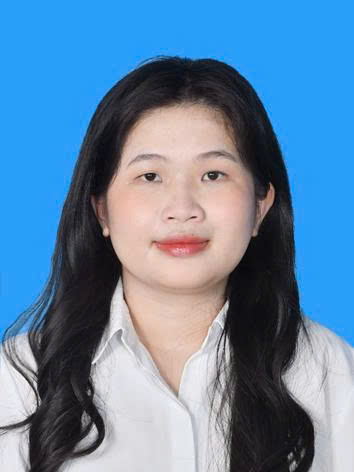
\includegraphics[
        width=2.2cm,
        height=2.7cm,
        keepaspectratio
    ]{assets/avt.jpg}
\end{minipage}

\end{tabularx}

\vspace{3pt}
\textcolor{rulecol}{\rule{\linewidth}{0.6pt}}

% ─── CAREER OBJECTIVE ────────────────────────────────
\section*{Career Objective}

{\small
Final-year Information Technology student with a strong foundation in
office applications, data processing, and software systems. Experienced
in using Microsoft Office, SQL, Power BI, and Python for data processing,
workflow automation, and reporting. Seeking to contribute to a professional
working environment by supporting office operations, data entry, document
processing, reporting, software support, and cross-department coordination.
}

% ─── EDUCATION ───────────────────────────────────────
\section*{Education}

\entry
{University of Transport Ho Chi Minh City (UTH)}
{10/2022 -- Expected 10/2026}
{Bachelor of Information Technology}

{\small
\begin{cvitems}

    \item GPA: 3.4 / 4.0

    \item \textbf{Academic Excellence Scholarship}
    -- Semester 1, 2025

    \item \textbf{Second Prize -- AI Track}
    -- UTH Student Scientific Research Conference 2025

\end{cvitems}
}

% ─── SKILLS ──────────────────────────────────────────
\section*{Skills}

{\small

\begin{tabularx}{\linewidth}{@{}lX@{}}

\textbf{Office Applications}
&
Proficient in Microsoft Word, Excel, and PowerPoint;
document preparation, spreadsheet processing, data consolidation,
and report preparation
\\[1.5pt]

\textbf{Data Processing}
&
Excel, SQL, PostgreSQL, SQL Server, Power BI;
data entry, data validation, consolidation, and analysis
\\[1.5pt]

\textbf{Systems \& Software}
&
Windows, software installation and configuration,
basic troubleshooting, service monitoring, and user support
\\[1.5pt]

\textbf{Automation}
&
Python scripting, data processing, and automation
of repetitive tasks
\\[1.5pt]

\textbf{Tools}
&
Git, Docker, Postman, VS Code, Power BI,
Jira, Confluence
\\[1.5pt]

\textbf{User Support}
&
Guiding users in software usage, handling requests,
troubleshooting issues, and coordinating with relevant departments
\\[1.5pt]

\textbf{English}
&
Technical document reading and basic professional communication

\end{tabularx}

}

% ─── WORK EXPERIENCE ─────────────────────────────────
\section*{Work Experience}

\entry
{Gotik Consulting -- Data Engineer}
{03/2026 -- 05/2026}
{Python \textbar{} Excel/Power BI \textbar{} PostgreSQL \textbar{} Airflow}

{\small
\begin{cvitems}

    \item Collected, validated, and processed business data
    from the Odoo system for reporting and analysis.

    \item Used Python and SQL to clean, process, and consolidate
    data from multiple sources.

    \item Developed reports and dashboards using Power BI
    to monitor operational performance.

    \item Automated recurring data processing tasks,
    reducing manual work and supporting regular reporting.

    \item Worked with PostgreSQL databases and collaborated
    on data and system-related issues.

\end{cvitems}
}

% ─── PROJECTS ────────────────────────────────────────
\section*{Selected Projects}

\entry
{Fall Detection -- Real-Time Fall Detection System}
{03/2026 -- 05/2026}
{Python \textbar{} FastAPI \textbar{} YOLOv8 Pose \textbar{} MediaPipe \textbar{} Transformer}

{\small
\begin{cvitems}

    \item Developed a software system for real-time camera data
    processing and dangerous behavior detection.

    \item Developed APIs and integrated data processing,
    AI, and alerting components.

    \item Achieved 97.8\% Mean Accuracy and integrated
    a Mobile App and Web Admin for monitoring and alerts.
    \item GitHub:
    \href{https://github.com/hohuynhnhu/Fall-Detection}
    {github.com/hohuynhnhu/Fall-Detection}
\end{cvitems}
}

\vspace{3pt}

\entry
{VehicleScan -- Smart Parking System}
{03/2025 -- 03/2026}
{Python \textbar{} YOLO \textbar{} CNN \textbar{} Firebase}

{\small
\begin{cvitems}

    \item Collected, validated, and managed datasets
    for system development.

    \item Developed and integrated AI models, APIs,
    databases, and application components.

    \item Won \textbf{Second Prize -- AI Track}
    at the UTH Student Scientific Research Conference 2025.
    \item GitHub:
    \href{https://github.com/LeKhang-cn22h/VehicleScanner.git}
    {github.com/LeKhang-cn22h/VehicleScanner.git}
\end{cvitems}
}

% ─── ADDITIONAL INFORMATION ──────────────────────────
\section*{Additional Information}

{\small

\begin{tabularx}{\linewidth}{@{}lX@{}}

\textbf{Soft Skills}
&
Attention to detail \textbar{} Responsibility \textbar{}
Problem solving \textbar{} Willingness to learn \textbar{}
Proactive working attitude
\\[2pt]

\textbf{Work Style}
&
Able to work independently and collaboratively,
handle requests, and complete tasks within deadlines
\\[2pt]

\textbf{Availability}
&
Available for full-time employment and flexible
working arrangements based on job requirements

\end{tabularx}

}

\end{document}



% \documentclass[10pt,a4paper]{article}

% % ─── Packages ─────────────────────────────────────────

% \usepackage{fontspec}
% \setmainfont{Times New Roman}

% \usepackage[top=1.1cm,bottom=1.1cm,left=1.55cm,right=1.55cm]{geometry}

% \usepackage{titlesec}
% \usepackage{enumitem}
% \usepackage{hyperref}
% \usepackage{xcolor}
% \usepackage{tabularx}
% \usepackage{graphicx}
% \usepackage{parskip}

% % ─── Colors ───────────────────────────────────────────

% \definecolor{primary}{RGB}{30,40,90}
% \definecolor{namecolor}{RGB}{0,120,180}
% \definecolor{accent}{RGB}{50,90,150}
% \definecolor{rulecol}{RGB}{200,205,220}
% \definecolor{gray}{RGB}{90,90,90}

% \hypersetup{
%     colorlinks=true,
%     urlcolor=accent
% }

% \pagestyle{empty}
% \setlength{\parskip}{0pt}

% % ─── Section ──────────────────────────────────────────

% \titleformat{\section}
%     {\normalsize\bfseries\color{primary}}
%     {}
%     {0em}
%     {}
%     [\vspace{1pt}\textcolor{rulecol}{\titlerule[0.6pt]}\vspace{1pt}]

% \titlespacing{\section}{0pt}{5pt}{2pt}

% % ─── Entry ────────────────────────────────────────────

% \newcommand{\entry}[3]{%
%     \noindent
%     \begin{tabularx}{\linewidth}{X r}
%         \textbf{\color{primary}#1} &
%         {\scriptsize\color{gray}#2}
%     \end{tabularx}\\[-2pt]
%     {\scriptsize\textit{\color{gray}#3}}
%     \vspace{1pt}
% }

% % ─── Compact list ─────────────────────────────────────

% \newenvironment{cvitems}{
%     \begin{itemize}[
%         leftmargin=1.15em,
%         topsep=0pt,
%         itemsep=0.5pt,
%         parsep=0pt,
%         partopsep=0pt
%     ]
% }{
%     \end{itemize}
% }

% % ═════════════════════════════════════════════════════

% \begin{document}

% % ─── HEADER ───────────────────────────────────────────

% \noindent

% \begin{tabularx}{\linewidth}{@{}X r@{}}

% % ─── Personal Information ───

% \begin{minipage}[c]{\linewidth}

%     {\LARGE\bfseries\color{namecolor} Ho Huynh Nhu}\\[2pt]

%     {\large\bfseries\color{primary}
%     IT Staff}\\[3pt]

%     {\scriptsize\color{gray}
%     20/10/2003
%     \enspace\textcolor{rulecol}{|}
%     \enspace (+84) 367 503 477
%     \enspace\textcolor{rulecol}{|}
%     \enspace
%     \href{mailto:hhnhu2003@gmail.com}{hhnhu2003@gmail.com}
%     \enspace\textcolor{rulecol}{|}
%     \enspace Ho Chi Minh City}\\[2pt]

%     {\scriptsize
%     \href{https://github.com/hohuynhnhu}
%     {github.com/hohuynhnhu}
%     \enspace\textcolor{rulecol}{|}
%     \enspace
%     \href{https://www.facebook.com/huynhnhu.ho.961}
%     {facebook.com/huynhnhu.ho.961}
%     }

% \end{minipage}

% &

% % ─── Avatar ───

% \begin{minipage}[c]{2.2cm}
%     \raggedleft
%     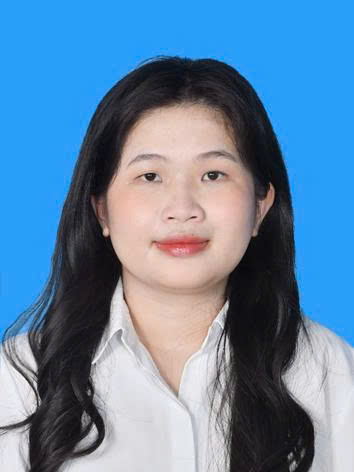
\includegraphics[
%         width=2.2cm,
%         height=2.7cm,
%         keepaspectratio
%     ]{assets/avt.jpg}
% \end{minipage}

% \end{tabularx}

% \vspace{3pt}

% \textcolor{rulecol}{\rule{\linewidth}{0.6pt}}

% % ─── CAREER OBJECTIVE ─────────────────────────────────
% % ─── CAREER OBJECTIVE ─────────────────────────────────

% \section*{Career Objective}

% {\small
% Final-year Information Technology student oriented toward IT and Python

% Backend development. Experienced in software systems, databases, APIs,

% troubleshooting, automation, and user support. Also familiar with

% AI/ML, Data Engineering, and operational dashboards.
% }

% % ─── EDUCATION ────────────────────────────────────────

% \section*{Education}

% \entry
% {University of Transport Ho Chi Minh City (UTH)}
% {10/2022 -- 10/2026}
% {Bachelor of Information Technology -- Completed coursework}

% {\small
% \begin{cvitems}

%     \item GPA: 3.4 / 4.0

%     \item \textbf{Excellent Scholarship} -- Semester 1, 2025

%     \item \textbf{Second Prize -- AI Track},
%     UTH Student Scientific Research Conference 2025

% \end{cvitems}
% }

% % ─── TECHNICAL SKILLS ─────────────────────────────────
% \section*{Technical Skills}

% {\small
% \begin{tabularx}{\linewidth}{@{}lX@{}}

% \textbf{IT \& Systems}
% &
% Windows, troubleshooting, system configuration, user support

% \\[1.5pt]

% \textbf{Backend \& API}
% &
% Python, FastAPI, Node.js, NestJS, RESTful API

% \\[1.5pt]

% \textbf{Database \& Data}
% &
% PostgreSQL, SQL Server, MongoDB, Firebase, Supabase,
% dbt, Airflow

% \\[1.5pt]

% \textbf{AI / Web / Mobile}
% &
% Machine Learning, Deep Learning, CNN, YOLO, Transformer,
% Nuxt.js, Vue 3, TypeScript, Flutter, Kotlin

% \\[1.5pt]

% \textbf{Tools}
% &
% Git, Docker, Postman, VS Code, Power BI, Jira, Confluence

% \\[1.5pt]

% \textbf{Office Skills}
% &
% Proficient in Microsoft Office

% \\[1.5pt]

% \textbf{English}
% &
% Technical document reading and basic professional communication

% \end{tabularx}
% }
% % ─── WORK EXPERIENCE ──────────────────────────────────

% \section*{Work Experience}

% \entry
% {Gotik Consulting -- Data Engineer}
% {Python \textbar{} dbt \textbar{} PostgreSQL \textbar{} Airflow \textbar{} Power BI}
% {03/2026 -- 05/2026}

% {\small
% \begin{cvitems}

%     \item Processed Odoo data for analysis and reporting.

%     \item Built Python + dbt pipelines on Neon PostgreSQL.

%     \item Automated hourly data workflows with Apache Airflow.

%     \item Developed Power BI dashboards for operational monitoring.

% \end{cvitems}
% }

% % ─── PROJECTS ─────────────────────────────────────────

% \section*{Featured Projects}

% \entry
% {Fall Detection -- Real-Time Fall Detection System}
% {Python \textbar{} FastAPI \textbar{} YOLOv8 Pose \textbar{} MediaPipe \textbar{} Transformer}
% {2025}

% {\small
% \begin{cvitems}

%     \item Developed a real-time fall detection system using
%     rule-based methods and Transformer.

%     \item Built the AI pipeline with MediaPipe, YOLOv8 Pose,
%     and a 30-frame $\times$ 200-feature sliding window.

%     \item Achieved 97.8\% mean accuracy with mobile and web
%     applications for alerts and management.

%     \item GitHub:
%     \href{https://github.com/hohuynhnhu/Fall-Detection}
%     {github.com/hohuynhnhu/Fall-Detection}

% \end{cvitems}
% }

% \vspace{3pt}

% \entry
% {VehicleScan -- Smart Parking System with IoT \& AI}
% {Python \textbar{} YOLO \textbar{} CNN \textbar{} Siamese \textbar{} ESP32 \textbar{} Firebase}
% {03/2025 -- 03/2026}

% {\small
% \begin{cvitems}

%     \item Built datasets and trained CNN, YOLO, and Siamese
%     Network models for vehicle recognition.

%     \item Integrated AI, IoT, sensor data, and rule-based logic
%     for smart parking management.

%     \item Achieved Second Prize -- AI Track at UTH 2025.

%     \item GitHub:
%     \href{https://github.com/LeKhang-cn22h/VehicleScanner.git}
%     {github.com/LeKhang-cn22h/VehicleScanner.git}

% \end{cvitems}
% }

% % ─── ADDITIONAL INFORMATION ───────────────────────────

% \section*{Additional Information}

% {\small
% \begin{tabularx}{\linewidth}{@{}lX@{}}

% \textbf{Soft Skills}
% &
% Problem-solving \textbar{} Willingness to learn \textbar{}
% Proactive troubleshooting \textbar{} Teamwork

% \\[2pt]

% \textbf{Other}
% &
% User support, software training, and system troubleshooting.

% \\[2pt]

% \textbf{Availability}
% &
% Willing to work shifts and adapt to job requirements.

% \end{tabularx}
% }

% \end{document}